\documentclass[a4paper,12pt]{article}

\usepackage[utf8]{inputenc}
\usepackage[english,russian]{babel}
\usepackage{longtable}
\usepackage{amsmath}
\usepackage{amsfonts}
\usepackage{amssymb}
\usepackage{cite}
\usepackage{graphicx}
\usepackage{epstopdf}
\usepackage{datetime}
\usepackage{indentfirst}
\usepackage{subfigure}
\usepackage[section]{placeins}
\usepackage{afterpage}
\usepackage{url}
\usepackage[unicode]{hyperref}
\usepackage{ucs}
\usepackage{listings}
\usepackage{microtype}
\usepackage{paralist}
\usepackage{multirow}
\usepackage{color}
\usepackage{xcolor}
\usepackage{float}
\usepackage{graphicx}
\usepackage{sectsty}
\usepackage{fancyhdr}
\usepackage{longtable}
\usepackage{appendix}
\usepackage{enumerate}
\usepackage{totcount}
\usepackage{verbments}
\usepackage{perpage}

\DeclareFontShape{OT1}{cmtt}{bx}{n}{<5><6><7><8><9><10><10.95><12><14.4><17.28><20.74><24.88>cmttb10}{}

\makeatletter
\renewcommand{\@biblabel}[1]{#1.}
\makeatother

\usepackage{geometry}
\geometry{left=2cm}
\geometry{right=2cm}
\geometry{top=2cm}
\geometry{bottom=2cm}

%% from bachelor-paper begin 
\fancyhf{}
\fancyfoot[C]{\normalsize \thepage}
\renewcommand{\headrulewidth}{0pt}
\renewcommand{\footrulewidth}{0pt}

%%Modifying captions for figures and tables:
\makeatletter
\long\def\@makecaption#1#2{%
\vspace{\abovecaptionskip}%
\sbox{\@tempboxa}{\large #1.~#2}
\ifdim \wd\@tempboxa >\hsize
{\large #1 --- #2}\par
\else
\global\@minipagefalse
\hbox to \hsize {\hfill {\large #1 --- #2}\hfill}%
\fi
\vspace{\belowcaptionskip}}

%% replaced with linespread? \renewcommand{\baselinestretch}{1.2}
\sectionfont{\Large}
\subsectionfont{\Large}
\subsubsectionfont{\Large}
\setlength{\belowcaptionskip}{6pt}
%% \makeatletter \renewcommand{\@biblabel}[1]{#1.\hfill}

\makeatletter 
\def\redeflsection{\def\l@section{\@dottedtocline{1}{1.5em}{7.8em}}} 
\renewcommand\appendix{\par 
\setcounter{section}{0}% 
\setcounter{subsection}{0}% 
\def\@chapapp{\appendixname}% 
\addtocontents{toc}{\protect\redeflsection} 
\def\thesection{\appendixname\hspace{0.2cm}\@Asbuk\c@section}} 
\makeatother 

\textwidth = 17cm
\oddsidemargin= 0 pt
\topmargin = -1cm
\headheight = 0cm
\headsep = 0cm
\textheight = 26.5cm

\newtotcounter[auxfile=totals.aux]{figurecnt}
\def\oldfigure{} \let\oldfigure=\figure
\def\figure{\stepcounter{figurecnt}\oldfigure}
\newtotcounter[auxfile=totals.aux]{bibcnt}
\def\oldbibitem{} \let\oldbibitem=\bibitem
\def\bibitem{\stepcounter{bibcnt}\oldbibitem}
\regtotcounter[auxfile=totals.aux]{page}

\linespread{1.3}

\newcommand{\td}{ (\#TODO) }
\newcommand{\todo}[1]{(\#TODO: #1)}
\newcommand{\doubletext}[2]{
	\noindent\begin{minipage}[b]{0.5\linewidth}
        #1
	\end{minipage}
	\noindent\begin{minipage}[b]{0.45\linewidth}
        \begin{flushright}
            #2
        \end{flushright}
    \end{minipage}
}

%\renewcommand{\theenumi}{\arabic{enumi}}
%\renewcommand{\labelenumi}{\arabic{enumi}}
%\renewcommand{\theenumii}{.\arabic{enumii}}
%\renewcommand{\labelenumii}{\arabic{enumi}.\arabic{enumii}.}
%\renewcommand{\theenumiii}{.\arabic{enumiii}}
%\renewcommand{\labelenumiii}{\arabic{enumi}.\arabic{enumii}.\arabic{enumiii}.}

\floatstyle{plain} % optionally change the style of the new float
\newfloat{code}{H}{myc}

\newcommand{\fu}[1]{\footnote{\url{#1}}}

%\definecolor{javapurple}{rgb}{0.25,0.35,0.9} % keywords
%% \definecolor{javapurple}{rgb}{0.1,0.1,0.1}


%\lstset{
%captionpos=b,
%breaklines=true,
%% basicstyle=\ttfamily,
%keywordstyle=\bfseries,
%% keywordstyle=\color{javapurple}\bfseries,
%% basicstyle=\ttfamily\color{black},
%% keywordstyle=\bfseries\color{keyword},
%showstringspaces=false,
%morekeywords={fun, val, var, import, object, uses, classpath, let, for, do, select, in, return, new, null, class}
%}

\MakePerPage{footnote}

\begin{document}
\def\figurename{Рисунок}

\begin{titlepage}
\large
\newpage

\begin{center}
Федеральное государственное бюджетное \\
образовательное учреждение высшего образования \\
Санкт-Петербургский национальный \\
исследовательский академический университет \\
российской академии наук
\end{center}

\begin{flushright}
\begin{minipage}[t][12em][c]{30ex}
\begin{center}
На правах рукописи \\
\medskip
Диссертация допущена к защите \\
Зав. кафедрой \\
\hrulefill \\
<<\hspace{2em}>> \hspace{1ex} \hrulefill \hspace{1ex} 2015 г.\\
\end{center}
\end{minipage}
\end{flushright}

\begin{center}
Диссертация \\
на соискание ученой степени \\
магистра \\
\end{center}

\noindent{Тема: Оптимизация байт-кода, генерируемого компилятором Kotlin}

\vspace{0.5cm}

\noindent{Направление: 03.04.01    –  Прикладные математика и физика}

\vspace{1.5cm}

\doubletext{Выполнил студент}{Д.С. Жарков}
\begin{center}
    \small (подпись)
\end{center}

\vspace{0.2cm}

\doubletext{Руководитель:}{А.А. Бреслав}
\begin{center}
    \small (подпись)
\end{center}

\vspace{0.2cm}

\doubletext{Рецензент: \\ к.ф.-м.н., доцент}{}
\begin{center}
    \small (подпись)
\end{center}

\vspace{1cm}

\begin{center}
    Санкт-Петербург

    2015 г.
\end{center}

\normalsize
\end{titlepage}


\addcontentsline{toc}{section}{Содержание}
\tableofcontents

\clearpage
\section*{Введение}
\addcontentsline{toc}{section}{\hspace{7mm}Введение}

Язык программирования Java на сегодняшний день является одним из самых популярных инструментов
разработки программного обеспечения. \footnote{\url{http://langpop.com/}}

Во многом своей популярности он обязан платформе JRE (Java Runtime Environment), включающей в себя
стандартную библиотеку языка и виртуальную машину Java (JVM), на которой исполняется скомпилированный код.
Именно наличие последнего пункта значительно облегчает задачу разработчика, решая такие непростые
проблемы,  как кросплатформенность, безопасность, управление памятью и отчасти производительность ПО.

Однако сам язык Java обладает рядом существенных недостатков: многословный и ``бедный'' синтаксис,
слабый вывод типов, развитие языка заторможено необходимостью сохранять обратную совместимость.

В связи с этим на рынке появляются новые языки, преодолевающие эти недостатки, но также
компилирующие исходный код программ в байткод для JVM и сохраняющие таким образом преимущества платформы.
Примером таких языков могут послужить Groovy, Scala, Kotlin, Clojure, Ceylon.

Поскольку для решений, базирующихся на платформе Java, нередко критичным фактором является
производительность и размер байткода приложения, то при сравнении этих языков в том числе следует
учитывать эти параметры кода, генерируемого их компиляторами.

Kotlin разрабатывается в компании JetBrains с 2010 года, а выпуск первой версии запланирован на середину 2015 года.

В рамках данной работы будет произведен анализ производительности байткода генерируемого его транслятором,
а также описаны решения, принятые для устранения найденных недочетов, такие как:
\begin{itemize}
    \item Устранение избыточного боксинга.
    \item Оптимизация генерации кода для сочетания операторов безопасного вызова и ``Elvis''.
    \item Оптимизация генерации оператора ``when'' для целочисленных констант, строк и классов-перечислений.
    \item Удаление мертвого кода.
    \item Решение проблемы с нарушением условий для <<On-stack-replacement>>.
\end{itemize}

%Квалификационная работа состоит из двух глав.

%В первой главе рассмотрены основные понятия предметной области, а также детализированы цели и задачи данной работы.

%Во второй рассмотрены уже существующие решения и приведены детали реализации полученной в рамках данной работы системы.

%В заключении описаны результаты работы и сформулированы перспективы дальнейшего развития системы.

\clearpage

\section*{Постановка задачи}

Главной целью данной работы --- улучшение производительности байт-кода, генерируемого компилятором
Kotlin.

Для ее достижения необходимо было решить следующие задачи:
\begin{itemize}
    \item Изучение подходов к производительности кода, реализованных в компиляторах других
    языков программирования для платформы Java.

    \item Измерение производительности байт-кода, генерируемого компилятором для различных
    синтаксических конструкций.

    \item Анализ, трактовка и классификация найденных в рамках стадии измерения проблем.

    \item Исследование оптимизаций, проводимых современными реализациями виртуальной машины
    Java, необходимое для определения критичности найденных проблем в генерируемом коде.

    \item Внедрение в компилятор изменений, способствующих решению найденных недостатков в коде
    и измерение производительности после этих изменений.
\end{itemize}

\clearpage

\section{Обзор предметной области}

\subsection{Виртуальная машина Java}

В этом разделе будет описан ряд особенностей, с которыми сталкиваются разработчики языков
программирования,компилирующихся в байткод виртуальной машины Java, далее именуемой \textit{JVM}.

В первую очередь следует подчеркнуть, что JVM --- абстрактная виртуальная машина, работающая
в соответствии со официальной спецификацией, выпущенной компанией Sun Microsystems и ныне
принадлежащей компании Oracle. %% spec link in biblio

У нее существует множество реализаций, в разной степени удовлетворяющих требованиям спецификации.
Известными примерами могут послужить: \textit{Hotspot} и \textit{JRockit} от Oracle, \textit{Azul Zing}
и \textit{Azul Zulu} --- относительно новые реализации от компании Azul Systems, \textit{Apache Harmony},
и многие другие.

\paragraph{Байт-код}

Основной сущностью, с которой работает JVM, является так называемый <<class-файл>>, как правило являющийся
бинарным отражением отдельного класса из исходного кода на языке Java. В нем закодированы основные
характеристики класса, такие как набор полей и методов, информация о его происхождении --- имя
скомпилированного файла, набор используемых строковых констант, и многое другое.

В рамках описания отдельного метода наиболее важной его частью является непосредственно код --- список
инструкций, которые должны быть исполнены виртуальной машиной при вызове этого метода.

Стоит отдельно упомянуть об особенностях набора инструкций JVM, существенно отличающих его
от низкоуровневых наборов, таких как x86 или ARM, которые реализованы для большинства современных
процессоров:
\begin{enumerate}
    \item Интерпретатор JVM представляет собой стековую машину, то есть операнды инструкций, как и
    их результаты, располагаются на стеке, причем в рамках работы одного вызова метода
    нельзя получить доступ к стеку родительского вызова.
    \item В наборе инструкций отсутствуют механизмы для ``прямого'' доступа к памяти процесса, по
    спецификации JVM состояние программы исчерпывается содержимым локальных переменных вызовов,
    полей объектов и статических полей классов.
    \item Единственным способом интерпроцедурного взаимодействия является инструкция вызова метода.
    Существует несколько вариантов таких инструкций, и выбор конкретной определяется сигнатурой
    вызываемого метода и контекстом вызова. Важной особенностью является наличие ``встроенной''
    обработки \textit{виртуальных} вызовов, % link to smth?
    когда выбор конкретного метода, зависит от конкретного класса объекта, на котором он вызывается.
    \item В большинстве реализаций JVM так или иначе реализован механизм верификации class-файлов,
    проверяющий их корректность. В частности проверке подлежат тела методов. Например верификатор
    может идентифицировать использование неинициализированной локальной переменной,
    которое в противном случае могло бы привести к неопределенному поведению прграммы.
\end{enumerate}

С точки зрения разработчика языка, целевой платформой для которого выбрана JVM, перечисленные
особенности могут стать, как достоинствами, так и недостатками. Как и любая другая абстракция,
виртуальная машина упрощает работу с абстрагируемым предметом, одновременно лишая некоторой
гибкости.

\paragraph{Динамическая трансляция}
%% [CFM+97] T. Cramer, R. Friedman, T. Miller, D. Seberger, R. Wilson,
%% and M. Wolczko. Compiling Java, just in time. IEEE Micro,
%% 17(3):3~3, May-June 1997.

%% Execution Characteristics of Just-In-Time Compilers
%% R. Radhakrishnany, J. Rubioy, L. K. Johny and N. Vijaykrishnanz

Как уже было сказано выше, с точки зрения спецификации байт-код методов интепретируется виртуальной
машиной Java.
Первые ее реализации были устроены именно так, однако быстро выяснилось,
что такой подход достаточно сильно влияет на производительность программ.

Во многом это связано с тем, что по сути на процессоре исполняется два потока: поток интепретации
и поток программы.
Кроме того интерпретируемые программы не могут оптимально использовать регистры процессора и с ними
менее удачно удается работать процессорным конвейерам из-за сложностей с предсказанием переходов.


%% http://www.cs.tufts.edu/comp/150IPL/papers/aycock03jit.pdf
Вполне естественным решением описанных проблем стала динамическая компиляция, далее именуемая
\textit{JIT}-компиляцией или просто \textit{JIT}. Суть ее заключается в том, что весь байт-код
метода или существенная его часть в момент работы приложения полностью транслируется в машинный код,
и затем передается к исполнению непосредственно на процессор.

Несмотря на то, что такой подход не был исторически новым, именно реализация динамической
компиляции в Hotspot очень сильно повлияла на судьбу интепретируемых языков, в том числе
сам термин --- JIT-компиляция --- стал общеупотребительным в литературе именно после выпуска Hotspot.%%\cite{}

В рамках данной работы очень важной хактеристикой JIT-компиляторов, поставляемых вместе
с популярными реализациями JVM, является факт наличия в них оптимизирующих подсистем. Например
разработчики Hotspot заявляют о следующих оптимизациях, производимых при компиляции:
%% https://wikis.oracle.com/display/HotSpotInternals/PerformanceTechniques
\begin{enumerate}
    \item Свертка константных выражений.
    \item Оптимизация проверок, которые должна производить JVM, таких как отслеживание вызова
    метода на null-объекте, при котором должно быть активировано соответствующее исключение.
    \item Так называемая <<размотка цикла>>. %% cite?
    \item Удаление недостижимого кода.
    \item Встраивание тел вызываемых методов в место вызова, в том числе оптимистичное встраивание
    полиморфных методов.
    \item Оптимизации основанные на информации, полученной при первичной интерпретации кода,
    с возможностью последующей декомпиляции. Оптимизации такого рода принципиально недоступны
    в компилируемых языка, так как на момент компиляции информация о профиле ее исполнения чаще
    всего отсутствует.
\end{enumerate}

По сути JIT-компиляторы популярных реализаций JVM так или иначе применяют весь набор оптимизаций,
использующихся в промышленных компиляторах языков, транслирующих программы в машинный код.
Из этого можно сделать два вывода:
\begin{itemize}
    \item Производительность кода на Java как минимум не сильно уступает аналогичному коду,
    написанному на компилируемом языке.
    \item Разработчикам языков для JVM в большинстве случаев не нужно дублировать соответствующие
    оптимизации при трансляции в байт-код, так как они будут произведены в рамках фазы
    динамической компиляции.

    Разумеется этот вывод может быть корректным только в случае, когда производительностью кода
    на фазе интерпретации можно пренебречь, что кажется вполне разумным, так как большая часть
    приложений, написанных для Java-платформы запускаются на достаточно длительное время,
    чтобы скомпилировать наиболее часто интерпретируемый код.
\end{itemize}

\subsection{Обзор существующих решений}

В рамках данного раздела будут рассмотрены и проанализированы решения, используемые в компиляторах
наиболее популярных языков языков программирования для платформы Java, а также дополнительно
будут рассмотрены отдельные приложения для постобработки сгенерированного байт-кода.

\subsubsection{Java}
Начинать обзор решений из компилятора языка Java следует с упоминания о том, что в принципе
существует несколько полноценных реализаций трансляторов, однако рассмотрены будут только версии,
распространяемые в комплекте Java Development Kit от Oracle, в силу их наибольшей популярности.

К сожалению непросто найти источник информации, исчерпывающе описывающий подходы к оптимизации,
используемые в компиляторах от Oracle, и который при этом можно было бы назвать хоть сколько-нибудь
авторитетным.

%% https://briangordon.github.io/2014/01/javac-optimizations.html
Наиболее адекватной и полной кажется статья [].
Предложенные в ней утверждения, кроме того, что они совсем не противоречат здравому смыслу,
еще регулярно подтверждались эмпирически при исследовании байт-кода, получаемого в результате
компиляции бенчмарков, написанных на Java. %% Ссылка на бенчмарки
Основные ее тезисы:
\begin{itemize}
    \item Для многих конструкций языка Java 6 существуют вполне очевидные правила их отображения
    в инструкции JVM, с помощью которых эти конструкции можно выразить.
    И в большинстве случаев компиляторы Java генерируют код весьма прямолинейно, следуя этим
    правилам, так, по что получаемому байт-коду можно зачастую однозначно определить вид исходного
    синтаксического дерева.
    \item В некотором смысле исключениeм является работа с константами:
    почти всегда, когда какое-то выражение может быть вычислено во время компиляции, в байт-коде
    будет уже результат этого вычисления.

    %% https://docs.oracle.com/javase/specs/jls/se8/html/jls-13.html
    Во многом это поведение описано в спецификации языка, и является полностью корректным,
    хотя в некоторых случаях неочевидным с точки зрения пользователя.

    \item Генерация последовательных применений оператора ``+'' для строк производится с помощью
    класса StringBuilder, что позволяет избежать избыточной аллокации и операций копирования памяти,
    которые неизбежно возникали бы в случае последовательных вызовов метода \textit{concat} у строк.

    \item Компилятор избегает генерацию заведомо мертвого кода, правда лишь в самых простых случаях.

    \item Некоторые простые оптимизации, применяемые при генерации условных операторов, упрощающие
    истиностные выражения в соответствии с законами де Моргана.
\end{itemize}

Кроме описанных в вышеуказанной статье пунктов стоит упомянуть несколько нетривиальную логику,
применяемую при генерации байт-кода для оператора ``switch'' для константных строк и более подробно
описанную в следующей главе. % link

Столь скудный набор оптимизаций, проводимых транслятором, вероятно связан с тем, что большая часть
работы с производительностью происходит уже во время работы программы на фазе JIT-компиляции.

% http://www.cis.upenn.edu/~bcpierce/courses/629/jdkdocs/tooldocs/win32/javac.html
% http://docs.oracle.com/javase/7/docs/technotes/tools/windows/javac.htm
% http://hg.openjdk.java.net/jdk6/jdk6/langtools/file/a9008b46db24/src/share/classes/com/sun/tools/javac/main/RecognizedOptions.java#l553
В пользу этого утверждения, в частности, говорит тот факт, что в документации к первым версиям
(до появления Hotspot) существовал флаг <<-O>>, позволяющий устанавливать уровень оптимизаций,
и который впоследствии из документации исчез.

Одним из выводов, который следует из этой части обзора --- код, генерируемый компилятором Java
может послужить эталоном для разработчика JVM-языка, как минимум в случае, когда
генерируемая конструкция достаточно проста, и присутствует в обоих языках: арифметические выражения,
простые условные операторы и т.д.
% http://www.mijnadres.net/published/Hotspot%20Optimizations.pdf
% https://www.usenix.org/legacy/events/jvm01/full_papers/paleczny/paleczny.pdf
% http://web.stanford.edu/class/cs343/resources/java-hotspot.pdf

В пользу последнего утверждения говорит также факт выполнения JIT-компилятором Hotspot
так называемых Peephole-оптимизаций[], шаблоны которых вполне вероятно могут быть приспособлены
именно для байт-кода, генерируемого компилятором Javac. Таким образом отступление от шаблонов
генерации Java потенциально может привести к ухудшению производительности.

\subsubsection{Java 8}
Одним из существенных нововведений, появившихся в относительно новой версии Java 8, стал лаконичный
синтаксис для анонимных функций.

В предыдущих версиях в случае необходимости определить функцию, параметризуемый некоторой другой
функцией, создавался интерфейс с одним методом, реализацию которого и следовало передать в первую
функцию.
% https://code.google.com/p/guava-libraries/wiki/FunctionalExplained
В популярной среди Java-разработчиков библиотеке <<guava>> для таких случае выделен общий
интерфейс, носящий недвусмысленное название Function[].

% https://docs.oracle.com/javase/specs/jls/se7/html/jls-15.html#jls-15.9.5
Чаще всего для реализации таких интерфейсов использовался громоздкий синтаксис анонимных классов[],
с помощью которого функцию-аргумент можно описать в месте вызова функции высшего порядка.
Примерно такой подход использовался и при генерации кода анонимных функций в новых языках для JVM:
для каждой из них генерировался отдельный синтетический класс с одним методом.

% http://cr.openjdk.java.net/~briangoetz/lambda/lambda-translation.html
При компиляции замыканий в Java 8 используется несколько другой подход: тело лямбда-функции
помещается в отдельный синтетический метод, располагаемый в том же классе, где происходит вызов
функции ожидающей реализацию интерфейса, а уже непосредственно класс-реализация генериуется
в момент первого вызова с помощью байт-код инструкции ``INVOKEDYNAMIC'', появишвшейся в поздних
версиях спецификаций JVM[]. % возможно стоит более подробно остановится?

Столь сложное и неочевидное решение, принятное инженерами Oracle, вряд ли существенно влияет на
производительность, так как фактически используется все тот же механизм интерфейсов и виртуальных
вызовов, намного сильнее такой подход влияет на число class-файлов в приложении.

Действительно, исходя из предположения об интенсивном использовании замыканий, генерация отдельного
class-файла в каждом месте вызова кажется избыточным, особенно учитывая, что не каждый из них
будет использован.

Однако у решения с ``INVOKEDYNAMIC'' есть как минимум один существенный недостаток: поддержка этой
инструкции существует только в версиях JVM младше седьмой, что сильно ограничивает возможность
использования такого кода в более старших версиях. В свою очередь попытки разработчиков языков
сохранить обратную совместимость например с версией JRE 1.6 зачастую являются не столько данью
консерватизму, сколько необходимостью для пользователей-разработчиков под Android, где по сей день
может быть использован только код, скомпилированный для устаревшей платформы.

\subsubsection{Scala}
Scala --- статически-типизированный мультипарадигменный язык программирования, компилируемый
в том числе под платформу Java. Системой типов, богатством синтаксических конструкций Scala
весьма сильно похож на Kotlin. В частности оба языка построены исходя из предположения
о повсеместном использовании функций высшего порядка, что сразу поднимает вопрос об эффективности
их реализации на уровне байт-кода.

В качестве основного источника информации о решениях, связанных с производительностью Scala,
автором была выбрана диссертация[] одного из разработчиков языка, который, как следует из статьи
занимался оптимизацией байт-кода, генерируемого компилятором.
Основные тезисы статьи будут рассмотрены в этом разделе.

\paragraph{Функции высшего порядка}

\newpage
\section{Измерения}
Одними из наиболее важных подзадач в рамках любой оптимизационной деятельности являются измерение,
трактовка результатов и определение наиболее важных для оптимизации мест.

В рамках данной главы будут изложены основные подходы, используемые при измерениях, результаты
измерений и их анализ.

\subsection{Корректность}
Измерение производительности программ следует производить с особой осторожностью, так как существует
множество различных факторов, в том числе случайных, влияющих на время их работы.

В случае программы для платформы Java, время ее работы во многом зависит от специфики работы
виртуальной машины.
В частности, изучая результаты измерений, следует уточнять:
\begin{itemize}
    \item Достаточно ли времени было у виртуальной машины для того, чтобы скомпилировать наиболее
    <<горячий>> код.

    Чаще всего непосредственно перед замером код бенчмарка запускается некоторое число раз с целью
    <<разогрева>> виртуальной машины.

    Это нужно не только для того, чтобы дать JVM возможность в принципе скомпилировать код, но и
    для накопления достаточного количества информации о профиле программы, чтобы адаптировать
    скомпилированный код для наиболее частых вариантов исполнения, в т.ч. для удачного расположения
    различных процедур в памяти.

    \item Насколько интенсивно запускаемый код аллоцирует динамическую память, достаточно ли ее.

    В случае жестких ограничений на память существенное время работы программы будет потрачено
    на сборку мусора, которая в особых случаях блокирует поток исполнения.

    \item Могла ли виртуальная машина доказать избыточность той части кода, которая подлежит
    измерению, и удалить соответствущие вычисления.

    В случае наличия такой возможности не может быть и речи о корректности измерений.
\end{itemize}

Для преодоления вышеописанных проблем все бенчмарки, описанные в данной работе, были реализованы
с помощью \textit{JMH}\fu{http://openjdk.java.net/projects/code-tools/jmh/}
--- каркаса для бенчмарков, разрабатываемого инженерами компании Oracle.

Каждый бенчмарк  представляет собой метод, отмеченный аннотацией ``Benchmark'', либо с пустым
набором параметров, либо принимающий объект класса ``Blackhole''.

Измерения производительности бенчмарка состоят из регулируемого числа итераций.
В рамках отдельной итерации код бенчмарка запускается несколько раз примерно в течение секунды,
после чего время работы вычисляется как среднее.

Результаты всех итераций рассматриваются, как выборка из нормального распределения с неизвестной
дисперсией, на основе которой вычисляется мат. ожидание, СКО, и доверительный интервал.

JMH предоставляет авторам бенчмарков ряд возможностей для контроля корректности измерений.
\begin{itemize}
    \item Пользователь может устанавливать число итераций разгогрева для каждого бенчмарка.
    Достаточность этого значения можно определить на основе анализа журнала компиляции HotSpot,
    который можно получить, запустив JVM с опцией ``-XX:+LogCompilation''.

    \item С помощью аннотации ``CompilerControl'' можно устанавливать будет ли конкретный метод
    скомпилирован или встроен JIT-компилятором, что позволяет моделировать различные варианты
    его поведения.

    \item JMH гарантирует, что если некоторое значение возвращено методом-бенчмарком или оно
    передано в качестве аргумента методу ``consume'' объекта ``Blackhole'', то виртуальная машина
    не сможет доказать избыточность кода, влияющего на это значение.

    \item В новых версиях JMH появилась возможность находить участки кода, которые исполняются
    дольше всего в процессе измерений.
    Вычисление наиболее <<горячих>> точек происходит с помощью инструмента ``perf''\fu{http://en.wikipedia.org/wiki/Perf_(Linux)},
    доступного для ОС Linux.

    Вывод результатов производится вместе с машинным кодом соответствующих участков на языке
    ассемблера.
    Это позволяет более точно оценить вклад тех или иных инструкций байт-кода в общее время работы
    бенчмарка.
\end{itemize}

\subsection{Условия проведения измерений}
\begin{itemize}
    \item \textbf{Модель ЦПУ:} Intel(R) Core(TM) i7-3540M CPU @ 3.00GHz
    \item \textbf{Операционная система:} Linux 3.11-2-amd64 \#1 SMP Debian 3.11.8-1 (2013-11-13) x86\_64 GNU/Linux
    \item \textbf{Реализация JVM:} Oracle Hotspot
    \item \textbf{Версии Java Runtime Edition:} 1.6.0\_45, 1.7.0\_51, 1.8.0
    \item \textbf{Ключи JVM:} -Xmx1024M -XX:+AggressiveOpt -XX:+DoEscapeAnalysis
\end{itemize}

\subsection{Бенчмарки}
В данном разделе представлено описание реализованных в рамках данной работы бенчмарков, указано
время их работы и проведен анализ недостатков в сгенерированном байт-коде.

Так как абсолютное время работы бенчмарка само по себе по сути не имеет смысла, для каждого из
них создан в некотом роде семантически эквивалетный эталон, производительность которого
с точки зрения автора должна быть близким к оригиналу.

Например при измерениях, нацеленных на проверку простых синтаксических конструкций, таким эталоном
может служить аналогичный код на Java, а при измерении времени работы стандартных функций высшего
порядка их код с заменой вызовов функционального аргумента на тело анонимной функции.

\subsubsection{АВЛ-дерево}
Одним из бенчмарков с существенно нетривиальным кодом стала реализация АВЛ-дерева, используемая
для решения задачи \textit{Stars}\fu{http://acm.timus.ru/problem.aspx?num=1028&locale=ru}.

По сути решение задачи сводится к последовательному добавлению элементов в дерево с запросом
порядкового номера добавленного элемента в отсортированном множестве.

В качестве <<идеального>> решения была использована реализация АВЛ-дерева, написанная автором
на Java, из которой с использованием автоматической конвертации была получена версия на Kotlin.

Большая часть полученного кода состоит из синтаксических конструкций, которые есть в обоих языках,
и единственным важным отличием стало использование в решении на Kotlin специальных операторов:
так называемые <<безопасный вызов>> и ``elvis''-оператор.

Семантика первого в целом имеет сходство с оператором <<точка>> из Java, но с дополнительной
проверкой выражения на котором происходит вызов на равенство ``null''.
\begin{pyglist}[language=kotlin]
x?.foo() // Safe-call
if (x != null) x.foo() else null
\end{pyglist}
В приведенном участке кода первая строка является примером безопасного вызова, а вторая
выражает его смысл.

Оператор ``elvis'' имеет семантику значения по умолчанию:
\begin{pyglist}[language=kotlin]
nullableInt ?: 0 // elvis
if (nullableInt != null) nullableInt else 0
\end{pyglist}

На практике нередко встречается их совместное использование.
Например при балансировке АВЛ-поддерева необходимо вычислить высоты каждого из двух поддеревьев,
причем при отсутствии поддерева его высота полагается равной нулю.
С помощью описанных выше конструкций высоту например левого поддерева можно выразить следующим
образом:
\begin{pyglist}[language=kotlin]
leftChild?.height ?: 0
\end{pyglist}

\paragraph{Результаты измерений}
Результаты измерений представлены в таблице ниже.
Параметр ``size'' --- количество добавляемых элементов, сами элементы --- случайные точки
на плоскости, но одинаковые в рамках каждого запуска.

\begin{table}[h]
\begin{center}
\begin{tabular}{|c|c|c|c|} \hline
Размер & Java & Kotlin & Фактор \\ \hline
100 & 19.412 $\pm$ 0.266 мкс & 30.687 $\pm$ 1.66 мкс & 1.581\\ \hline
1000 & 300.055 $\pm$ 2.397 мкс & 476.807 $\pm$ 4.243 мкс & 1.589\\ \hline
100000 & 78.686 $\pm$ 3.14 мс & 132.768 $\pm$ 3.938 мс & 1.687\\ \hline
\end{tabular}
\caption{Результаты бенчмарка <<АВЛ-дерево>>}
\end{center}
\end{table}

Из результатов измерений следует, что версия на Kotlin работает примерно в $1.7$ раз хуже, чем
аналогичный код на Java.
После анализа байт-кода обоих версий было сделано предположение, что наибольший вклад в ухудшение
производительности вносит именно вышеупомянутое сочетание операторов.
Для подтверждения гипотезы была релизована еще одна версия на Kotlin, в которой вместо
безопасного вызова и elvis-оператора используется обычный условный оператор вида:
\begin{pyglist}[language=kotlin]
if (leftChild != null) leftChild.height else 0
\end{pyglist}

Результаты модифицированной версии бенчмарка:

\begin{table}[h]
\begin{center}
\begin{tabular}{|c|c|c|c|} \hline
Размер & Java & Kotlin & Фактор \\ \hline
100 & 19.412 $\pm$ 0.266 мкс & 23.801 $\pm$ 0.367 мкс & 1.226\\ \hline
1000 & 300.055 $\pm$ 2.397 мкс & 331.832 $\pm$ 2.14 мкс & 1.106\\ \hline
100000 & 78.686 $\pm$ 3.14 мс & 87.722 $\pm$ 4.974 мс & 1.115\\ \hline
\end{tabular}
\caption{Результаты бенчмарка <<АВЛ-дерево>> (упрощенная версия)}
\end{center}
\end{table}

Такая версия бенчмарка существенно приблизилась в плане производительности к эталону, таким образом
подтвердив предположение.
Это побудило к более тщательному исследованию производительности кода, генерируемого
для этих операторов, результаты которого изложены в следующем разделе.

\subsubsection{Безопасный вызов и elvis-оператор}
Для уточнения производительности вышеописанного сочетания был реализован следующий микро-бенчмарк:
\begin{itemize}
    \item Определен класс ``Data'' с единственным полем, содержащим целое число
    \item Перед запуском создается массив фиксированного размера, который заполняется с некоторой
    вероятностью либо нулевой ссылкой, либо объектом класса ``Data'' со случайным числом.
    \item Код бенчмарка берет последовательно элементы массива, и для каждого из них
    вычисляет выражение:
    \begin{pyglist}[language=kotlin]
    obj?.x ?: 1
    \end{pyglist}
    \item В качестве эталонного бенчмарка вычисляется эквивалентное выражение с помощью простого
    условного оператора:
    \begin{pyglist}[language=kotlin]
    if (obj != null) obj.x else 1
    \end{pyglist}

    \item Вероятность нулевой ссылки меняется с шагом $0.4$ от $0.1$ до $0.9$.
\end{itemize}

\begin{table}[h]
\begin{center}
\begin{tabular}{|c|c|c|c|} \hline
$p$ & Эталон (мкс) & Бенчмарк (мкс) & Фактор \\ \hline
0.1 & 4.693 $\pm$ 0.036 & 9.131 $\pm$ 0.126 & 1.946\\ \hline
0.5 & 7.103 $\pm$ 0.078 & 7.138 $\pm$ 0.263 & 1.005\\ \hline
0.9 & 4.561 $\pm$ 0.043 & 4.738 $\pm$ 0.047 & 1.039\\ \hline
\end{tabular}
\caption{Результаты бенчмарка "Безопасный вызов и elvis" \newline (p --- вероятность нулевой ссылки)}
\end{center}
\end{table}

Из результатов можно сделать следующие выводы:
\begin{itemize}
    \item Для сочетания операторов безопасного вызова и elvis действительно генерируется байт-код
    уступающий в производительности байт-коду семантически аналогичного условного выражения.

    \item Так как сильнее всего это проявляется когда большая часть объектов не является нулевыми
    ссылками ($p = 0.1$), проблемное место находится в ветвлении для где `obj` не равен `null`.
\end{itemize}

%\begin{verbatim}
                %aload_1 // Загрузка `obj` на стек     
                %dup         
                %ifnull l1
                %getfield x
                %invokestatic  java/lang/Integer.valueOf() // Боксинг
                %goto          l3
                %l1: pop         
                %aconst_null 
                %// начало кода elvis-оператора
                %l2: dup         
                %ifnull l3
                %invokevirtual java/lang/Number.intValue() // Распаковка
                %goto          l4
                %l3: pop         
                %iconst_1
                %l4: ...
%\end{verbatim}

\begin{figure}
\begin{center}
    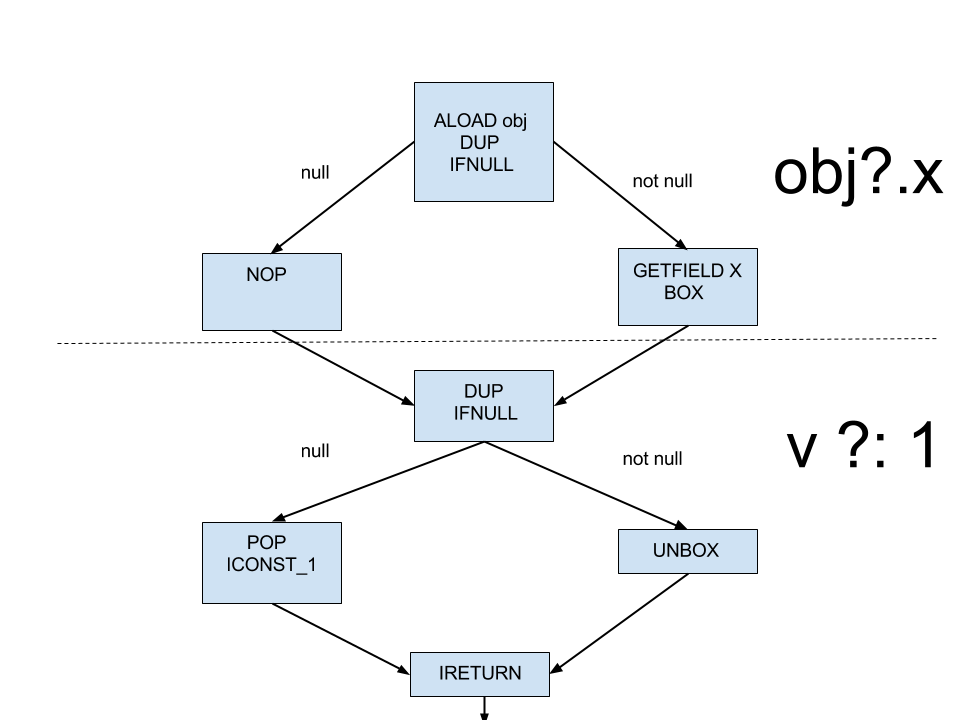
\includegraphics[scale=0.4]{../resources/safecall_elvis.png}
\end{center}
\caption{Блок-схема байт-кода для выражения ``return (obj?.x ?: 1)''}
\label{sc:elvis}
\end{figure}

Примерная блок-схема байт-кода бенчмарка изображена на рисунке \ref{sc:elvis}.
Часть, расположенная выше пунктирной линии описывает генерацию безопасного вызова:
\begin{itemize}
    \item На стек загружается переменная ``obj'', ее значение копируется с помощью инструкции
    ``DUP'', и копия проверяется на равенство ``null''.
    \item В случае если ``obj'' является нулевой ссылкой, то лежащее на вершине стека значение
    тоже нулевая ссылка.
    Иначе на стеке лежит объект ``obj'', у которого берется значение в поле ``x'' и упаковывается.
\end{itemize}

Таким образом обеспечивается контракт безопасного вызова, и на вершине стека находится либо нулевая
ссылка, либо упакованное значение поля.

Боксинг в данном случае необходим, так как ситуация, когда при одном потоке исполнения в ячейке
стека значение примитивного типа, а при другом --- ссылка, запрещена спецификацией виртуальной
машины\cite{JVMSpec}.

Вторая часть блок-схемы иллюстрирует байт-код для elvis-оператора:
\begin{itemize}
    \item Значение, лежащее на вершине стека, копируется и проверяется на равенство нулевой ссылке.
    \item В случае, если оно является нулевой ссылкой, то его копия снимается со стека и
    загружается значение по умолчанию --- целочисленная константа <<1>>.

    Иначе не стеке лежит объект класса ``java.lang.Integer'', из которого и получается значение
    с помощью вызова метода ``intValue'', на блок-схеме этот вызов отмечен для простоты, как
    ``UNBOX''.
\end{itemize}

Понятно, что байт-код этих операторов по отдельности наиболее очевидным образом выражает
их семантику, и выразить их еще проще в рамках спецификации JVM, пожалуй, не представляется
возможным.
Однако их сочетание ни в коей мере оптимальным не кажется.

\begin{figure}
\begin{center}
    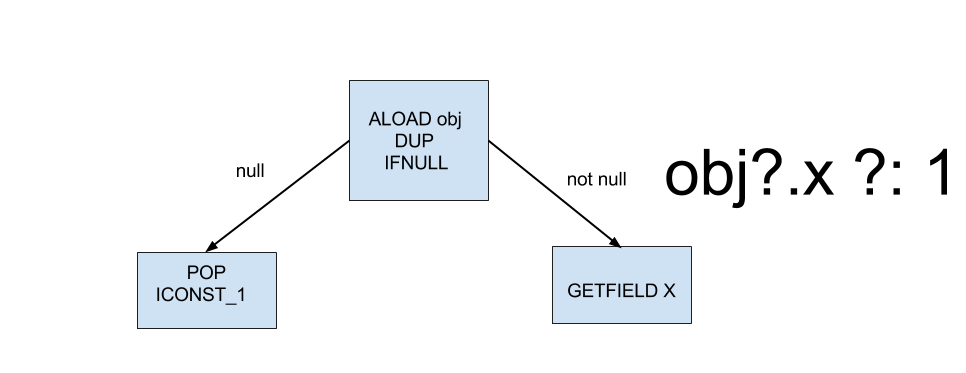
\includegraphics[scale=0.4]{../resources/safecall_elvis_optim.png}
\end{center}
\caption{Блок-схема байт-кода для выражения ``return (obj?.x ?: 1)'' (оптимальный вариант)}
\label{sc:elvisOpt}
\end{figure}

Наиболее кратким вариантом трансляции кажется изображенный на рисунке \ref{sc:elvisOpt}:
\begin{itemize}
    \item Переменная ``obj'' загружется на стек, создается ее копия, и сравнивается с нулевой
    ссылкой.
    \item Если значение является нулевой ссылкой, то его копия снимается со стека, и загружается
    значение по умолчанию.
    Иначе на вершине стека хранится объект, у которого берется значение поля ``x''.
\end{itemize}

При такой генерации отсутствуют операции боксинга, что, как выяснилось в рамках измерений,
хуже всего влияет на производительность вышеописанного байт-кода.

Оптимизации, направленные на решение найденной проблемы, описаны в разделе . % TODO: \ref

\subsubsection{Оператор when}
Оператор ``when'' в Kotlin является в некотором смысле расширением оператора ``switch'' в Java.
Если последний имеет ограниченный набор типов значений, для которых его можно использовать, то
``when'' определен для любых типов, и кроме сравнения на равенство его можно использовать для
проверки принадлежности чисел интервалу, или как некоторую разновидность паттерн-матчинга:

\begin{pyglist}[language=kotlin]
    when(x) {
        1, 2, 3, parseInt(s) -> print(1)
        in 4..1000 -> print(2)
        is String -> print(3)
        else -> print(4)
    }
\end{pyglist}
В случае неконстантных выражений-условий наиболее разумным способом генерации кажется простая
последовательная проверка истинности проверяемых выражений.
При трансляции байт-код для ``when'' аналогичен байт-коду цепочки ``if-else'' операторов,
производительность которых в Kotlin так или иначе не хуже аналогов из Java.

Важно отметить, что оператор ``switch'' можно применять только для набора выражений, которые можно
вычислить во время компиляции.
Причем при трансляции в байт-код используются специальные инструкции \textit{tableswitch} и
\textit{lookupswitch}\cite{JVMSpec}.
Их объединяет общая семантика:
\begin{itemize}
    \item Они параметризуются отображением из набора целых чисел в указатели на другие инструкции
    метода.
    \item При исполнении инструкции интерпретатор снимает с вершины стека число и совершает
    соответствующий переход.
\end{itemize}

Различия заключаются в том, что
\begin{itemize}
    \item \textit{tableswitch} параметризуется интервалом $[high..low]$.
    Для каждого целочисленного значения из этого интервала должна быть задана метка перехода,
    а кроме этого указатель на инструкцию по умолчанию.

    Таким образом размер этой инструкции линейно зависит от ширины интервала.
    \item \textit{lookupswitch} параметризуется отсортированным набором пар значений и меток
    перехода.

    Размер такой инструкции зависит линейно от числа значений.
\end{itemize}

Несмотря на то, что в спецификации не указана трудоемкость выполнения этих инструкций, из формата
их описания понятно, что ``tableswitch'' может быть исполнен за $O(1)$ прямым вычислением индекса
следующей инструкции, а ``lookupswitch'' может быть реализован на основе бинарного поиска и
работать за $O(log\ n)$.

На момент начала данного исследования эти инструкции не использовались в компиляторе Kotlin,
в связи с чем возникла необходимость оценить проигрыш в производительности для случая констант
времени компиляции по сравнению с Java.

Для этого был реализован следующий набор бенчмарков:
\begin{itemize}
    \item Функции с операторами ``switch''/``when'' с набором из последовательных значений
    для сопоставления из интервала $1..20$.
    Каждое условное ветвление представляет из себя оператор ``return'' с уникальным целым числом.
    Предполагается в Java такой ``switch'' транслируется в инструкцию ``tableswitch'',
    предзначначенную как раз для последовательных интервалов.

    \item Бенчмарки, аналогичные предыдущим, но с еще одним условным значением, значительно
    выходящим за пределы интервала $1..20$ --- $0$.
    Предполагается, что здесь должна быть использована инструкция ``lookupswitch'', подходящая
    для разреженных интервалов.

    \item Бенчмарки где операторы ``switch'' и ``when'' применяются для значений класса-перечисления
    (enum).
    Всего в классе объявлено 100 значений, в условном операторе используется 50 с четными номерами.

    \item Бенчмарки, где операторы ``switch'' и ``when'' применяются для строк.
    В качестве выражений для сопоставления использовались строки с вида <<ABCDEFGHIJKLMNO[i]>>,
    где $i$ --- порядковый номер в интервале $1..50$.

    В качестве аргументов использовались случайно выбранные строки из этого же множества.
\end{itemize}

Бенчмарки запускались в цикле на 1000 значений, выбранных случайным образом.

\begin{table}[h]
\begin{center}
\begin{tabular}{|c|c|c|c|} \hline
Разреженность & Java (мкс) & Kotlin (мкс) & Фактор \\ \hline
1..20 & 4.281 $\pm$ 0.018 & 7.8 $\pm$ 0.131 & 1.822\\ \hline
1..20, 100500 & 5.554 $\pm$ 0.077 & 7.524 $\pm$ 0.065 & 1.355\\ \hline
\end{tabular}
\caption{Сравнение производительности операторов switch/when для целочисленных констант}
\end{center}
\end{table}

\begin{table}[h]
\begin{center}
\begin{tabular}{|c|c|c|c|} \hline
Тип & Java (мкс) & Kotlin (мкс) & Фактор \\ \hline
Enum & 10.501 $\pm$ 0.167 & 13.885 $\pm$ 0.037 & 1.322\\ \hline
Строки & 21.667 $\pm$ 0.205 & 81.931 $\pm$ 1.671 & 3.781\\ \hline
\end{tabular}
\caption{Сравнение производительности операторов switch/when для классов перечислений и строк}
\end{center}
\end{table}

Из результатов измерений видно, что разница в производительности различных реализаций
составляет от $1.3$ до $3.7$ раз.

А так как использование константных выражений в подобного рода операторах является довольно
распространенной в программировании практикой, то при генерации следует рассмотреть такой
отдельно и при наличии возможность использовать оптимизирующие инструкции.

Подробности реализации оптимизации для данного случая можно рассмотреть в разделе . %% TODO: \ref

\subsubsection{Встраивание функций}
Изначально предполагается, что производительность встроенных функций должна быть аналогична
производительности кода, полученного при ручном встраивании.

Например код вызова:
\begin{pyglist}[language=kotlin]
    arrayOfInts.count { element -> element > 0 }
\end{pyglist}

где функция ``count'' определена как
\begin{pyglist}[language=kotlin]
    inline fun IntArray.count(predicate: (Int) -> Boolean): Int {
        var count = 0
        for (element in 0..size) {
            if (block(element)) {
                count++
            }
        }
        return count
    }
\end{pyglist}
не должен существенно уступать по производительности коду:
\begin{pyglist}[language=kotlin]
        var count = 0
        for (element in 0..size) {
            if (element > 0) {
                count++
            }
        }
\end{pyglist}

Однако, как было отмечено в разделе \ref{section:scala} добиться этого не слишком просто.

Для проверки влияния встраивания функций на производительность был реализован ряд бенчмарков,
каждый из которых проверяет эффективность различных функций стандартной библиотеки Kotlin
для работы с коллекциями:
\begin{itemize}
    \item ``count'' --- возвращает число элементов коллекции, удовлетворяющих заданному
    предикату-аргументу.
    \item ``filter'' --- возвращает ``ArrayList'' из значений коллекции, удовлетворяющих заданному
    предикату-аргументу.
    \item ``fold'' --- выполняет левоассоциативную свертку элементов коллекции, используя
    в качестве бинарной операции функцию-аргумент.
\end{itemize}

В качестве аргумента для функций использовался целочисленный массив, заполенный случайными числами.
Бенчмарки запускались для размеров массивов: 100, , 00.

В качестве эталонной версии использовался код, встроенный <<вручную>>, как в примере выше.

\begin{table}[h]
\begin{center}
\begin{tabular}{|c|c|c|c|} \hline
Размер & Эталон & Встроенная версия & Фактор \\ \hline
100 & 87.968 $\pm$ 0.78 нс & 348.255 $\pm$ 11.299 нс & 3.959\\ \hline
10000 & 18.401 $\pm$ 0.251 мкс & 78.05 $\pm$ 0.981 мкс & 4.242\\ \hline
1000000 & 3.715 $\pm$ 0.021 мс & 8.565 $\pm$ 0.098 мс & 2.306\\ \hline
\end{tabular}
\caption{Сравнение производительности вызова ``count \{ it \% 2 == 0 \}'' и аналогичного кода, встроенного вручную}
\label{bm:count}
\end{center}
\end{table}

\begin{table}[h]
\begin{center}
\begin{tabular}{|c|c|c|c|} \hline
Размер & Эталон & Встроенная версия & Фактор \\ \hline
100 & 598.23 $\pm$ 5.017 нс & 711.114 $\pm$ 8.057 нс & 1.189\\ \hline
10000 & 98.655 $\pm$ 1.764 мкс & 121.1 $\pm$ 1.74 мкс & 1.228\\ \hline
1000000 & 11.868 $\pm$ 0.529 мс & 13.68 $\pm$ 1.195 мс & 1.153\\ \hline
\end{tabular}
\caption{Сравнение производительности вызова ``filter \{ it \% 2 == 0 \}'' и аналогичного кода, встроенного вручную}
\label{bm:filter}
\end{center}
\end{table}

\begin{table}[h]
\begin{center}
\begin{tabular}{|c|c|c|c|} \hline
Размер & Эталон & Встроенная версия & Фактор \\ \hline
100 & 27.676 $\pm$ 0.159 нс & 477.024 $\pm$ 3.474 нс & 17.236\\ \hline
10000 & 2.784 $\pm$ 0.021 мкс & 47.563 $\pm$ 0.57 мкс & 17.084\\ \hline
1000000 & 301.023 $\pm$ 1.828 мкс & 4.69 $\pm$ 0.031 мс & 15.581\\ \hline
\end{tabular}
\caption{Сравнение производительности вызова ``fold(0) \{ sum, x -> sum + x \}'' и аналогичного кода, встроенного вручную}
\label{bm:fold}
\end{center}
\end{table}

Из результатов (см. таблицы \ref{bm:count}, \ref{bm:filter}, \ref{bm:fold}) видно, что код
встроенных версий от $1.$ до $16$ раз менее производительный, чем в принципе мог бы быть.

При профилировании с помощью плагина ``perfasm'' для JMH было установлено, что наибольший вред
для производительности приносит избыточный боксинг, оставшийся в качестве артефакта от встраивания
параметрически-полиморфного метода ``invoke'' анонимного класса (см. раздел \ref{section:lambda}).
Эта проблема так или иначе уже была поднята в рамках исследования\cite{ScalaDragos} и обсуждена
в рамках раздела \ref{section:scala}.

Наименее всего это влияет на бенчмарк ``filter'', так как значения все равно должны быть запакованы
перед сохранением в ''ArrayList``.

Сильнее всего разница заметна в случае бенчмакр ``fold'', где вычисляется сумма элементов массива.
Это связано с тем, что более чистый байт-код версии, написанной вручную, позволяет компилятору
HotSpot выполнить т.н. размотку цикла, суммирая в каждой итерации по $10$ элементов массива.

Оптимизации, связанные с улучшением производительности встраиваемых функций, описаны в разделе . %% TODO: \ref

\subsubsection{Замена на стеке}
Одной из разновидностей динамической трансляции, реализованной в Hotspot, является так называемая
<<Замена на стеке>> или ``On stack replacement''(OSR), описанная в \cite{HotspotServer}.

В отличие от простой версии JIT-компиляции, когда оптимизированная версия метода используется
только при следующем его вызове, OSR позволяет перейти к исполнению скомпилированного кода в рамках
уже начатого вызова.

Это может быть полезно, например, в случае, когда метод, содержащий цикл с трудоемкими вычислениями,
начал исполняться в режиме интерпретации, и при этом число итераций этого цикла достаточно велико.
В этом случае, если количество итераций преодолело порог-параметр ``OnStackReplaceThreshold'',
код метода компилируется, и в рамках следующей итерации исполняется оптимизированная версия.

Как следует из примера выше, для измерения времени работы необходим бенчмарк, содержащий долго
работающий цикл.
Такими бенчмарками могут послужить описанные в предыдущем разделе при больших размерах массива,
во время анализа работы которых было обнаружено странное поведения при компиляции метода на стеке.

А именно, функция ``foldBenchmark'' вида:
\begin{pyglist}[language=kotlin]
    fun foldBenchmark(): Int {
        return array.fold(0) { (x, y) -> x + y }
    }
\end{pyglist}

за разумное время компилировался <<на стеке>>, и хотя время его работы примерно в 20 раз
отличалось от эталонного, это можно было объснить избыточным боксингом.

Однако байт-код для семантически схожей функции ``foldBenchmarkOSR'' оказался в десятки раз менее
производительным, чем предыдущий (см. таблицы \ref{bm:foldOSR}, \ref{bm:foldOSR2}).
\begin{pyglist}[language=kotlin]
    fun foldBenchmarkOSR(bh: Blackhole) {
        bh.consume(array.fold(0) { (x, y) -> x + y })
    }
\end{pyglist}

Особенно интересным фактом в результатах измерений является то, что производительность второй
версии не уступает обычной версии ``fold'' при малых размерностях.
А кроме того, такое различие наблюдается только при запуске на версиях Hotspot 1.7, 1.8, когда
время на Hotspot 1.6 не отличается (см. таблицу \ref{bm:foldOSR3}).

\begin{table}[h]
\begin{center}
\begin{tabular}{|c|c|c|c|} \hline
Размер & Эталон & foldBenchmarkOSR & Фактор \\ \hline
100 & 27.832 $\pm$ 0.341 нс & 595.958 $\pm$ 4.061 нс & 21.413\\ \hline
10000 & 2.773 $\pm$ 0.006 мкс & 95.095 $\pm$ 0.832 мкс & 34.297\\ \hline
1000000 & 301.701 $\pm$ 4.575 мкс & 114.624 $\pm$ 2.055 мс & 379.925\\ \hline
\end{tabular}
\caption{Сравнение производительности вызова ``foldBenchmarkOSR'' и аналогичного кода, встроенного вручную (версия Hotspot 1.7)}
\label{bm:foldOSR}
\end{center}
\end{table}

\begin{table}[h]
\begin{center}
\begin{tabular}{|c|c|c|c|} \hline
Размер & fold & foldBenchmarkOSR & Фактор \\ \hline
100 & 594.34 $\pm$ 6.472 нс & 595.958 $\pm$ 4.061 нс & 1.003\\ \hline
10000 & 100.181 $\pm$ 0.584 мкс & 95.095 $\pm$ 0.832 мкс & 0.949\\ \hline
1000000 & 11.28 $\pm$ 0.063 мс & 114.624 $\pm$ 2.055 мс & 10.162\\ \hline
\end{tabular}
\caption{Сравнение производительности вызова ``foldBenchmarkOSR'' и аналогичного кода из бенчмарка ``fold'' (версия Hotspot 1.7)}
\label{bm:foldOSR2}
\end{center}
\end{table}

\begin{table}[h]
\begin{center}
\begin{tabular}{|c|c|c|c|} \hline
Размер & fold & foldBenchmarkOSR & Фактор \\ \hline
100 & 477.024 $\pm$ 3.474 нс & 478.739 $\pm$ 5.202 нс & 1.004\\ \hline
10000 & 47.563 $\pm$ 0.57 мкс & 47.482 $\pm$ 0.422 мкс & 0.998\\ \hline
1000000 & 4.69 $\pm$ 0.031 мс & 4.685 $\pm$ 0.051 мс & 0.999\\ \hline
\end{tabular}
\caption{Сравнение производительности вызова ``foldBenchmarkOSR'' и аналогичного кода из бенчмарка ``fold'' (версия Hotspot 1.6)}
\label{bm:foldOSR3}
\end{center}
\end{table}
Причем различия заметны только при больших размерностях задачи, что и дает повод искать корни
проблемы в трансляции <<на стеке>>, так как вероятно метод не успевает запуститься достаточное
число раз для полной компиляции.

После анализа журналов компиляции было определено, что компилятор Hotspot версий 7 и 8
не поддерживает для <<замены на стеке>> циклы, в начале которых стек виртуальной машины не пуст.

\begin{quote}
\begin{verbatim}
<failure reason='OSR starts with non-empty stack'/>
<failure reason='OSR starts with non-empty stack' phase='compile'/>
\end{verbatim}

\captionof{floatquote}{Фрагмент журналов компиляции}
\end{quote}

\begin{verbatim}

\end{verbatim}

Такая ситуация, когда цикл начинается с непустым стеком принципиально невозможна в Java, где
цикл не может быть частью выражения.

Однако проблема может возникнуть в языках, таких как Scala и Kotlin, где любые операторы являются
также и выражениями, то есть пример, описанный ниже --- корректная синтаксическая конструкция:
\begin{pyglist}[language=kotlin]
    fun foldBenchmarkOSR(bh: Blackhole) {
        foo().bar(for (i in 1..100) { print(i) })
    }
\end{pyglist}

Так как результат выражения ``foo()'' должен быть вычислен до выполнения аргумента вызова
``bar()'', то перед началом цикла на вершине стека находится результат ``foo()'', что и приводит
к невозможности проведения замены на стеке.

Несмотря на то, что использование цикла внутри выражения не имеет смысла, аналогичная ситуация
возникает и в разумных случаях, таких как в бенчмарке ``foldBenchmarkOSR'', где перед началом
цикла встроенной функции ``fold'' на стеке загружена переменная ``bh''.

Аналогичная проблема возникает и при встраивании функций в Scala\fu{https://issues.scala-lang.org/browse/SI-8057}.
Оптимизации, связанный с найденной проблемой описаны в разделе . %% TODO: \ref


\newpage
\nocite{*}
\bibliographystyle{bplain}
\bibliography{biblio}

\end{document}

